\documentclass[letterpaper, 11pt]{article}

\usepackage{amsmath}
\usepackage[final]{graphicx}
\usepackage[left = 1.5in, right =1.5in, top = 1.25in, bottom = 1.25in]{geometry}
\usepackage{booktabs}
\usepackage{tabularx}
\usepackage{longtable}


\title{FAnalyze v0.1 \\User's Manual}
\author{Dan Valente\\\small{Mitra Lab}\\\small{Cold Spring Harbor Laboratory}}
\date{\today}

\begin{document}
\maketitle

\section{Introduction}

FAnalyze is a suite of functions written in Matlab to aid in the analysis of animal behavior in the
Open Field.   It was written and tested primarily for fly exploratory behavior in a circular arena,
and a description and illustration of the measures calculated by FAnalyze can be found in Ref.\
\cite{valente1}.  FAnalyze assumes that the user has tracked the (x,y) location of the animal to
obtain the trajectory that the animal took over the course of the experiment.  FAnalyze smooths the
data, calculates the animal's velocity, and allows one to segment space and speed based on hard
thresholds.  With this inaugural version, FAnalyze only allows for segmentation into circular zones
(it is assumed that the Open Field arena is circular). FAnalyze then allows the user to calculate
and display probability distributions of the relevant variables to obtain a quantitative phenotypic
characterization of the exploratory behavior.  Please note that these calculations --- the
probability distributions --- are the focus of the program.

Although it has been rigourously tested, being that this is version 0.1, please be aware that
multiple bugs may still exist in FAnalyze.  If you find them, feel free to fix them (if you are
Matlab savvy), or send an email to the author.  To use FAnalyze, a basic working knowledge of
Matlab is assumed.


\section{Placing FAnalyze in the Matlab path}
In order to use FAnalyze, the FAnalyze folder must first be placed in the Matlab path.

\begin{enumerate}
\item Open Matlab.
\item Select \textbf{File $>>$ Set Path\ldots} from the toolbar.  The Set Path dialogue will open up.
\item Click on the \textbf{Add Folder\ldots} button.
\item Find the FAnalyze directory and select the \textbf{functions} folder. Click \textbf{OK}.  The path and name of the
FAnalyze functions folder should show up in the Matlab search path window.
\item Click \textbf{Save}, and then click \textbf{Close}. FAnalyze is now ready to use.  To test if
it is installed correctly, \texttt{help FAnalyze} in the Matlab command window. If an error is
obtained upon this command, the folder was not correctly installed, so try to re-install. If the
installation worked, you will be able to open the program or use any of the functions regardless of
what directory you are currently in.
\end{enumerate}


\section{The FAnalyze GUI}
The FAnalyze graphical user interface (GUI) was written to facilitate use of the analysis functions
for quick data exploration.  It is not intended for large scale data analysis---the individual
FAnalyze Matlab functions are best for this---although the user may find the GUI useful in
high-throughput studies.
\begin{figure}
    \centering
    \hspace{-0cm}
    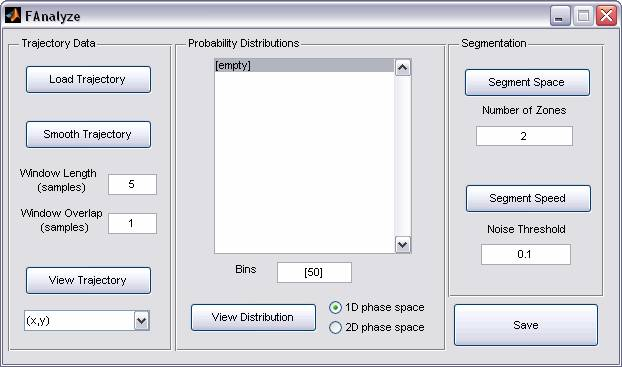
\includegraphics[bb= 0.0 0.0 622.0 367.0 clip=true, scale = 0.7]{GUI.jpg}
    \caption{The FAnalyze GUI}
    \label{GUI}
\end{figure}
The interface is shown in Fig.\ \ref{GUI} and is divided into three general sections: Trajectory
Data, Probability Distributions, and Segmentation. The functionality of these sections is described
below.


\subsection*{Loading a Trajectory}

To begin, the user must load a trajectory file for analysis by clicking the \textbf{Load
Trajectory} button. FAnalyze assumes that the data is contained in a \texttt{.mat} file.  Within
that file \emph{must} be variables labeled \texttt{x}, \texttt{y}, and \texttt{t} describing the
spatial coordinates and time of every point in the trajectory. FAnalyze permits analysis of only
one file per session.  Once the file is loaded, a message is displayed in the Command Window
informing the user of the chosen file's name.

\subsection*{Instructions for Smoothing}

Due to jitter in the object's location caused by non-translational object movements and artifacts
of the tracking method, it is typically good practice to smooth the resulting trajectory. The
smoothing is executed using the function \texttt{runline} from the Chronux neural data analysis
software package (http://www.chronux.org), which performs a local linear regression on the
data\footnote{\texttt{runline} is included with FAnalyze, so having Chronux is not a pre-requisite
for use of this program.}.

\begin{enumerate}
 \item Select the length of the running window (in samples) to be used in the smoothing process.
 \item Select the step-size (in samples) that the window will take as it moves across the data (also
 known as the Window Overlap.)  Enter these numbers into the appropriate boxes.
 \item Click the \textbf{Smooth Trajectory} button.  In the Command Window, a message informs the user that the smoothing process is underway\footnote{Smoothing may take a long time, depending on the length of the trajectory.}.  When smoothing has finished, a message
 will be displayed declaring a successful completion of the smoothing algorithm.
\end{enumerate}
Because smoothing can significantly eliminate fluctuations in the data, one is advised to
investigate the effects of changing the smoothing parameters on the resulting trajectory.  This
will allow you to decide what amount of fluctuations are physically relevant in your videos. For
instance, if the data is smoothed too drastically, a short but visible stop of the object can be
entirely smoothed into an apparent movement!

\subsection*{Viewing the Trajectory}

Once the data is smoothed, the user is able to view the resulting trajectory.  Simply select the
plot of interest from the pull-down menu in the Trajectory Data section and click \textbf{View
Trajectory}. The user has access to view the following data (note that a circular arena is assumed,
hence the availability of data in polar coordinates):

\begin{tabular}{l r}
\texttt{(x,y)} & The complete position trajectory\\
\texttt{x} & The x-coordinate as a function of time\\
\texttt{y} & The y-coordinate as a function of time\\
\texttt{r} & The radial coordinate as a function of time \\
\texttt{theta} & The angular coordinate as a function of time\\
\texttt{vx} & The x-velocity as a function of time\\
\texttt{vy} & The y-velocity as a function of time\\
\texttt{v} & The speed as a function of time\\
\texttt{vtheta} & The direction of the velocity vector as a function of time
\end{tabular}

\subsection*{Creating and Viewing Probability Distributions}

The philosophy behind  FAnalyze is as follows\footnote{This is adapted from Ref.\ \cite{valente1}}:
We regard the trajectory as a stochastic process $\mathbf{x}(t)$.  This process would be fully
characterized if the joint distributions $P(\mathbf{x}(t_1), \mathbf{x}(t_2), \ldots
,\mathbf{x}(t_n))$ were specified for all choices of time points $(t_1,t_2, \ldots ,t_n )$.
Unfortunately, the full distribution, $P(\mathbf{x}(t_1), \mathbf{x}(t_2), \ldots ,x(t_n))$, is
difficult (if not impossible) to measure. However, by examining joint distributions of position and
velocity along with distributions of path curvature, reorientation angle, and event durations, we
can obtain a convenient summary of the animal's behavior in the arena and its interaction with the
environment.

The distributions are estimated using histograms of the data, so it is recommended that the
organism be studied for a long period of time for ``clean-looking" distributions (a ``good" length
of time will depend on the activity of the animal and the frame rate that the video was taken at).
These probability histograms are calculated with the functions \texttt{ProbDist1D},
\texttt{ProbDist2D}, and \texttt{JointDist}.

 When examining histogram estimates of probability distributions, one needs to exercise care about phase space factors in order to obtain
accurate estimates.  For example, if the animal is moving in two dimensions, the probability
density for the speed $v$ along with the phase space factors is given by $p(v)vdvd\theta$ (where
$\theta$ is polar angle of the point $(v_x,v_y)$ in velocity space). Therefore, binning data in
bins of size $\Delta v\Delta\theta$ would yield an estimate for $p(v)v$. When this is the case, we
eliminate the need to divide by $v$ (which could be an unstable calculation for small $v$) by
binning in $v^2$, since $p(v)vdvd\theta \sim p(v^2/2)d(v^2/2)d\theta$. For one-dimensional motion,
such as movement along the arena boundary, there are no phase space factors and it is sufficient to
bin the data in $v$. FAnalyze allows the user to select whether to calculate the distributions
assuming a 1D or 2D phase space.   For 2D phase space calculations, the user should take note of
the non-constant bin widths of these histograms.

Therefore, as soon as the data is smoothed (as well as when the data is segmented), the Probability
Distributions list box will become populated with the variables that are available for analysis.
The naming convention for variables in the list box is described in Appendix A. To calculate and
view the probability distributions of interest, proceed as follows:
\begin{enumerate}
\item For a single variable marginal distribution, highlight the variable of interest by clicking
on it.  For a joint distribution of two variables, select the first variable of interest, hold down
the CTRL button on the keyboard, and select the second variable of interest.
\item Enter the \textbf{Bins} to use for the calculation. This field will accept any bin description that the Matlab \texttt{hist} or \texttt{hist3} commands accept.  See
the help files of those functions for details, and make sure that brackets commas and other
necessary puncuation are used. Also note that no other options available to \texttt{hist} or
\texttt{hist3} are available in the FAnalyze functions with this release (v0.1).

As an example, if you wish to calculate a joint distribution having 100 bins in the first variable
and 150 in the second, you would enter: \texttt{[100 150]}.  If, instead you wanted bin centers
from 0 to 10 in steps of 0.1 for the first variable, and bin centers from 2 to 4 in steps of 0.3
for the second you would enter: \texttt{ \{[0:0.1:10] [2:0.3:4]\}}. (Note the curly brackets).

\item  Select whether the variable of interest exists in a one or two-dimensional phase space (see above).

\item Click the \textbf{View Distribution} button.  The distribution will be calculated and a plot
of the distribution will be displayed.
\end{enumerate}
Every calculation that is performed is held in memory until FAnalyze is closed.  At any point in
time, you may click the Save button to save your calculations (structure of data is described
below).  Unfortunately, at this point, the user cannot access the calculated data from the command
window until after the data is saved and reloaded.

\subsection*{Segmenting Space}

Often, an examination of the joint distributions $p(x,v)$ or $p(r,\theta)$ will show that the
animal has a spatial preference for some part of the arena.  FAnalyze allows the user to segment
the arena into any number of circular spatial ``zones."  Please note that only concentric circular
zones are allowed (or, rather, toroidal zones).  To segment space:
\begin{enumerate}
\item Enter the \textbf{Number of Zones} that you wish to segment the arena into.
\item Click the \textbf{Segment Space} button.  A window will pop up asking the user to input
relevant information.
\item Input the location of the threshold defining the boundary between zones 1 and 2, in terms of the radial distance from center.  Enter names for these zones. Click \textbf{OK}.
\item If more than two zones are requested, another window will pop up asking for similar
information.  Make sure that the first zone name in this window is the same as the second name in
the last window and that the second threshold is larger than the first; otherwise, you will get an
error (zone 2 must have a consistent name, and the second threshold must be further than the first
threshold).
\item Repeat this for all the zones you requested.
\item Once the segmentation is finished, a message will be displayed in the command window, and the
Probability Distributions list box will be populated with variables available for analysis.
\end{enumerate}

\subsection*{Segmenting Speed}

Similar to the spatial distributions, when examining the speed distribution $p(v)$, the user may
find that the distribution appears to be a mixture of a few different types of motion.  Because of
this, investigators often find it useful to segment the speed into distinct modes of motion. In
FAnalyze, speed segmentation is performed almost exactly as the space segmentation. To segment
speed:
\begin{enumerate}
\item Enter the \textbf{Noise Threshold} seen in your data.  The noise threshold is the lowest speed that
you can accurately resolve.  It can be obtained by examining the speed vs.\ time plot and noting
the maximum speed attained in regions where the animal is visibly stationary.  Velocity and speed
points below this threshold are assigned a value of 0.
\item Click the \textbf{Segment Speed} button.  A window will pop up asking the user to input
relevant information \emph{for each spatial zone}.
\item Input the location of the threshold defining the boundary between segments 1 and 2, in terms of the absolute speed.  Enter names for these segments. Click \textbf{OK}.
\item If more than two segments are requested, another window will pop up asking for similar
information.  Make sure that the first segment name in this window is the same as the second name
in the last window and that the second threshold is larger than the first; otherwise, you will get
an error (segment 2 must have a consistent name, and the second threshold must be further than the
first threshold).
\item Repeat this for all the segments and zones you requested.
\item FAnalyze now segments the data according to the user's requests, as well as calculating where
the animal has stopped (points below the noise threshold).  Stops are considered a ``segment."
\item Once the segmentation is finished, a message will be displayed in the command window, and the
Probability Distributions list box will be populated with variables available for analysis.
\end{enumerate}

\subsection*{Saving the Data}
To save the data from the session as a \texttt{.mat} file, click on the \textbf{Save} button in the
lower right-hand corner of FAnalyze. The user is asked to choose a location and a filename in which
to save.  The
data is saved as two cells, \texttt{traj} and \texttt{P}.\\

\noindent\texttt{traj} is a 1 x $N$ cell, where $N$ is the number of zones in the arena.  The
$i^{\text{th}}$ cell contains a structure with the trajectory information from that zone.  Within
that structure, each variable is a cell itself containing structures for each speed segment. For
example, data from the second zone is accessed by typing \texttt{traj\{2\}} and is organized as
follows:
\begin{verbatim}
traj{2} =
     zone_label: {`CZ'}
     seg_label: {`all'  `stops'  `NZS'  `FSS'}
             t: {[1x1 struct]  [1x1 struct]  [1x1 struct]  [1x1 struct]}
             x: {[1x1 struct]  [1x1 struct]  [1x1 struct]  [1x1 struct]}
             y: {[1x1 struct]  [1x1 struct]  [1x1 struct]  [1x1 struct]}
             r: {[1x1 struct]  [1x1 struct]  [1x1 struct]  [1x1 struct]}
         theta: {[1x1 struct]  [1x1 struct]  [1x1 struct]  [1x1 struct]}
            vx: {[1x1 struct]  [1x1 struct]  [1x1 struct]  [1x1 struct]}
            vy: {[1x1 struct]  [1x1 struct]  [1x1 struct]  [1x1 struct]}
             v: {[1x1 struct]  [1x1 struct]  [1x1 struct]  [1x1 struct]}
        vtheta: {[1x1 struct]  [1x1 struct]  [1x1 struct]  [1x1 struct]}
           tau: {[1x1 struct]  [1x1 struct]  [1x1 struct]  [1x1 struct]}
         kappa: {[1x1 struct]  [1x1 struct]  [1x1 struct]  [1x1 struct]}
          beta: {[1x1 struct]}
\end{verbatim}
The labels are fairly self explanatory. Note that \texttt{beta} can only be calculated if all the
points in the trajectory are considered.

The $j^{\text{th}}$ entry of each variable's cell contains a structure with a single field.  This
field is called \texttt{data}.  So, if one is interested in extracting the x-position of the
organism in zone \texttt{`CZ'} (the second zone), while the organism walked in speed segments
labeled by \texttt{`FSS'} (the fourth segment), one would type

\begin{verbatim}
traj{2}.x{4}.data
\end{verbatim}

The probability histograms are saved in the \texttt{P} cell.  \texttt{P} is a 1 x M cell, where M
is the number of times the View Distributions button was pressed during the session.  Each entry of
the cell contains a structure that is organized as follows:
\begin{verbatim}
P{1} =
    label: `x_Full Arena_all'
    phase_opt: `phase1D'
    data: [1x50 double]
    bins: [1x50 double]
\end{verbatim}

The field \texttt{label} is the name of the variable from which the probability distribution was
calculated. \texttt{phase\_opt} denotes whether the user chose to calculate the distribution
assuming a 1D or 2D phase space. \texttt{data} contains the bin-by-bin data from the calculated
histogram, and \texttt{bins} contains the bin centers.  If an error occurs, the entry is completely
empty.

Admittedly, this seems complicated, but the author felt it was a decent way to organize the data
file.

\section{Known Problems}

There is only one known problem with FAnalyze at this point.  Please be aware that you cannot
choose to segment speed and \emph{then} segment space.  You must segment space first and
\emph{then} segment speed. You can, however, select to only segment speed or only segment space.


\section{Concluding Comments}

For those who wish to use the functions from the Matlab command line, complete descriptions of
their use and workings can be found in the Matlab help files; simply type \texttt{help
function\_name}.  Describing them in detail here would be superfluous.  The scripts are also
commented, and as such, they should be relatively easy to follow. Suggestions for improvements to
the algorithms, the GUI or the coding style are highly encouraged!  Comments on the ease of use of
the GUI and functions are also important for refining this program.  Since this is v0.1, FAnalyze
needs quite a bit of testing in order to find all of the bugs (pun intended).  Until then, please
check and double-check any results that you obtain from this program, and make sure that they make sense! \\

\noindent Enjoy!


\section{Appendix A: Variable Naming Convention}
There are eleven variables that are available for analysis in FAnalyze.  They are:\\

\begin{tabular}{l r}
\texttt{x} & The x-coordinate as a function of time\\
\texttt{y} & The y-coordinate as a function of time\\
\texttt{r} & The radial coordinate as a function of time \\
\texttt{theta} & The angular coordinate as a function of time\\
\texttt{vx} & The x-velocity as a function of time\\
\texttt{vy} & The y-velocity as a function of time\\
\texttt{v} & The speed as a function of time\\
\texttt{vtheta} & The direction of the velocity vector as a function of time\\
\texttt{tau} & Duration of speed segments\\
\texttt{kappa} & Curvature of the path \\
\texttt{beta} & Reorientation angle
\end{tabular}\\

In the list box, these variable names are followed by the zone name and the speed segment name as
given by the user.  For example, for a zone named \texttt{`RZ'} and a speed segment within that
zone named \texttt{`FSS'}, the speed would appear as \texttt{v\_RZ\_FSS}.  For the full arena, the
label is automatically called (appropriately) \texttt{`Full Arena'}. If all the velocity points are
included the speed segment label is \texttt{`all'}.  Therefore, after smoothing and before any
segmentation, the variables in the list contain the label \texttt{`\_Full Arena\_all'}.



\begin{thebibliography}{9}
\bibitem{valente1}Valente, D., Golani, I., and P.P. Mitra, ``Analysis of the trajectory of \emph{Drosophila
melanogaster} in a circular open field arena." PLoS ONE 2(10), e1083
doi:10.1371/journal.pone.0001083, (2007)
\bibitem{valente2}Valente, D., Wang H., Andrews P., Saar S., Tchernichovski O., Benjanimi, Y., Golani I. and
P.P. Mitra, ``Characterization of animal behavior through the use of audio and video signal
processing." IEEE Multimedia, 14 (2), 32-41, (2007)
\end{thebibliography}

\end{document}
